
\begin{enumerate}
\item The inequality constraints are
  \[
  \begin{array}{rrcl}
    - x_1 & + x_2 &\leq& 2, \\
     x_1 & + x_2 &\leq& 4, \\
    - x_1 &    &\leq& 0, \\
           & - x_2 &\leq& 0. \\
  \end{array}
  \]
\item 
  Each of the four constraints defines a half-plane, and the
  intersection of the half-planes gives the polyhedron in $\R^2$. We
  draw first the lines defined by the equality version of the
  constraints: 
  \[
  \begin{array}{rrcl}
    - x_1 & + x_2 &=& 2, \\
     x_1 & + x_2 &=& 4, \\
    - x_1 &    &=& 0, \\
           & - x_2 &=& 0. \\
  \end{array}
  \]
  In order to identify on which side of the line is the half-plane, we
  use the gradient with the opposite sign. Indeed, the gradient of a
  function indicates the direction in which the function
  increases. Here, as the function must be less or equal to a
  constant, we need the direction in which the function decreases.

  For instance, for the first constraint, the gradient is the first
  row of the matrix $A$. Written as a column vector, it is:
  \[
\rvect{-1 \\ 1}.
\]
Therefore, the direction that shows which side of the line is feasible is
  \[
\rvect{1 \\ -1}.
\]
The other directions are obtained in the same way:
\[
d_1 = \rvect{1 \\ -1}, \; d_2 = \rvect{-1 \\ -1}, \; d_3 =
\cvect{1\\ 0}, \; d_4 = \cvect{0 \\ 1}.
\]

\begin{center}
    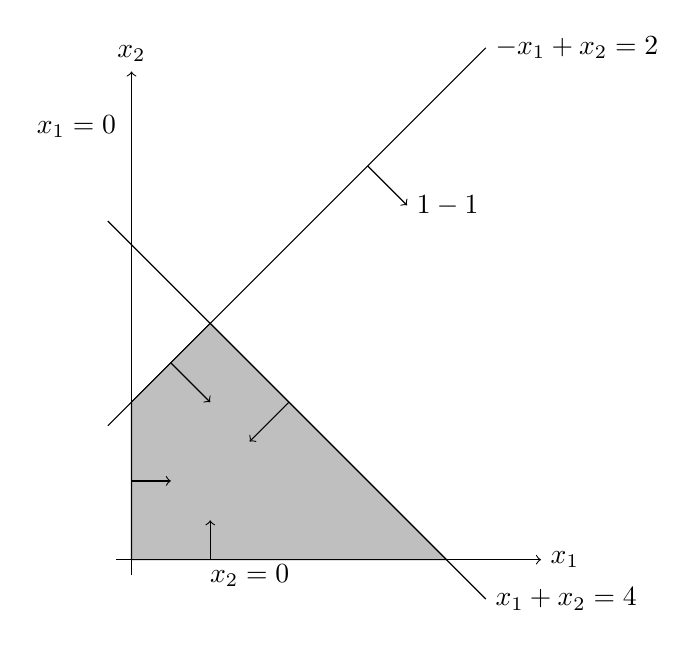
\begin{tikzpicture}[domain=-0.3:4.5]
      \draw[->] (-0.2,0) -- (5.2,0) node[right] {$x_1$};
      \draw[->] (0,-0.2) -- (0,6.2) node[above] {$x_2$};
      \draw[color=black] plot (\x,\x+2) node[right] {$-x_1 + x_2 = 2$};
      \draw[color=black] plot (\x,4-\x) node[right] {$x_1 + x_2 = 4$};
      \node at (1.5,-0.2) {$x_2 = 0$};
      \node at (-0.7,5.5) {$x_1 = 0$};
      \draw[fill=lightgray]  (0,0) -- (0,2) -- (1,3) -- (4,0) -- cycle;
      \draw[->] (3,5) -- ++(0.5,-0.5) node[right] {$\rvect{1 \\ -1}$};
      \draw[->] (0.5,2.5) -- ++(0.5,-0.5) ;
      \draw[->] (2,2) -- ++(-0.5,-0.5);
      \draw[->] (1,0) -- ++(0,0.5);
      \draw[->] (0,1) -- ++(0.5,0);
%      \draw[pattern=vertical lines]  (0,0) -- (0,2) -- (1,3) -- (4,0) -- cycle;
	\end{tikzpicture}
\end{center}
    \item In order to write the standard form of the polyhedron, we
      need to include the slack variables. As there are 4 inequality
      constraints, we need 4 slack variables:
    \begin{equation}
    \mathcal{P} = \{x \in \R^2, x^s \in \R^4 \mid Ax + x^s = b, x^s \geq 0\}.
    \end{equation}
We now have 6 variables. The set of constraints characterizing the
polyhedron is:
\[
    \begin{array}{rrrrrrr}
        -x_1  & + x_2 & +x_3 &      &      &   &  = 2, \\
         x_1 &  + x_2 &      & +x_4 &      &   & = 4, \\
        -x_1 &        &      &     &  +x_5 &  & = 0, \\
             & -x_2   &      &     &       &+x_6 & = 0, \\
         x_1  &       &      &     &       &     & \geq 0, \\               
              & x_2   &      &     &       &     & \geq 0, \\               
              &       & x_3  &     &       &     & \geq 0, \\               
              &       &      & x_4 &       &     & \geq 0, \\               
              &       &      &     & x_5   &     & \geq 0, \\               
              &       &      &     &       & x_6 & \geq 0. \\               
    \end{array}
    \]
\end{enumerate}
